\documentclass[tikz,border=5pt]{standalone}
\usepackage{tikz}
\usetikzlibrary{calc}

\begin{document}
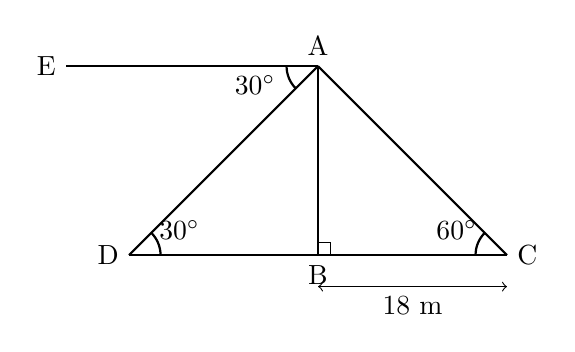
\begin{tikzpicture}[scale=0.8]
    \coordinate (B) at (2,0);
    \coordinate (A) at (2,3);
    \coordinate (C) at (5,0);
    \coordinate (D) at (-1,0);
    \coordinate (E) at (-2,3);
    
    \draw[thick] (D) node[left]{D} -- (C) node[right]{C};
    \draw[thick] (B) node[below]{B} -- (A) node[above]{A};
    \draw[thick] (A) -- (C);
    \draw[thick] (A) -- (D);
    \draw[thick] (A) -- (E) node[left]{E};
    \draw (2,0.2) -- (2.2,0.2) -- (2.2,0);
    
    % Angle arc EAD = 30° at A (from AE direction to AD direction)
    \draw[thick] ($(A)+(180:0.5)$) arc (180:225:0.5);
    \node at (1,2.7) {$30^{\circ}$};
    
    % Angle arc ADB = 30° at D (from DA direction to DB direction)
    \draw[thick] ($(D)+(0:0.5)$) arc (0:45:0.5);
    \node at (-0.2,0.4) {$30^{\circ}$};
    
    % Angle arc ACB = 60° at C (from CA direction to CB direction)
    \draw[thick] ($(C)+(135:0.5)$) arc (135:180:0.5);
    \node at (4.2,0.4) {$60^{\circ}$};
    
    \draw[<->] (2,-0.5) -- (5,-0.5) node[midway, below]{18 m};
\end{tikzpicture}
\end{document}